\title{Umbau eines \textsc{Detroit Electric Cars}}
\team{%
    Yanick Frei,
		Marc Müller}

\client{Urs Jäger}

\coach{%
    Felix Jenni}

\fssummary{
    Ein Elektrofahrzeug aus dem Jahre 1918 wurde auf Lithium-Ionen-Batterien umgerüstet. Zeitgleich wurde die Funktion des Fahrzeuges, insbesondere die Stufenschaltung, analysiert und instand gestellt.}

\fsgraphics{
    \begin{minipage}{0.47\textwidth}
        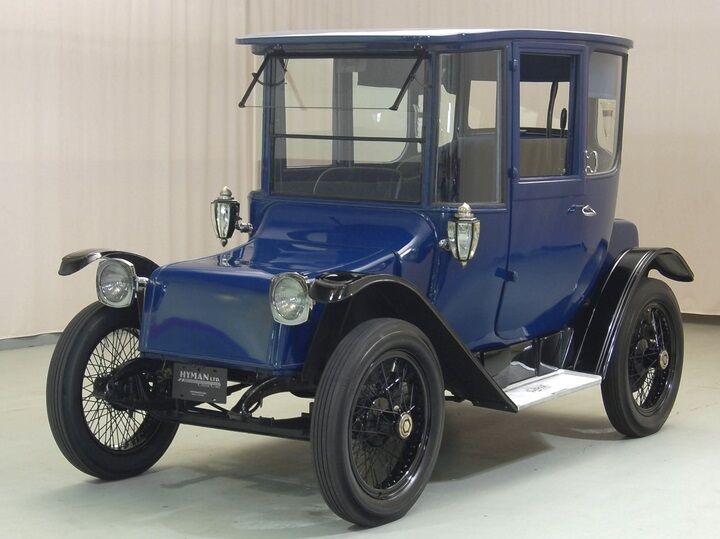
\includegraphics[height=54mm]{images/Detroit.jpg}
        \graphicscaption{Das Fahrzeug im aktuellen Zustand}
    \end{minipage}%
    \begin{minipage}{0.53\textwidth}
        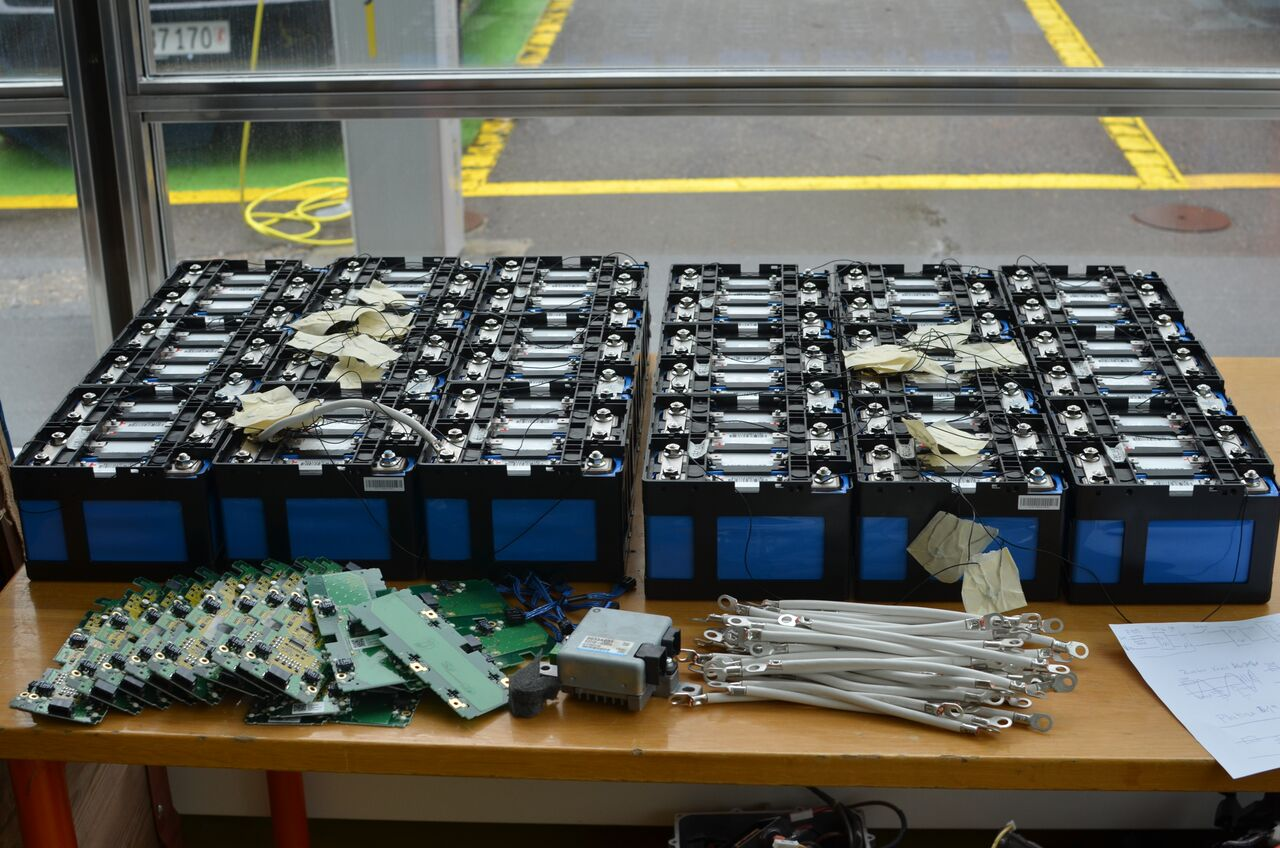
\includegraphics[height=54mm]{images/Batterie.jpg}
        \graphicscaption{Die Batterie vor dem Einbau}
    \end{minipage}
}

\fscontent{
    \section{Das Fahrzeug}
		Beim Fahrzeug handelt es sich um einen \textsc{Detroit Electric Car} aus dem Jahre 1918. Zu dieser Zeit waren Elektrofahrzeuge weit verbreitet und insbesondere bei Frauen beliebt, da das mühselige Anwerfen und die Abgase von Verbrennungsmotoren entfielen.
		
		Über mehrere Umwege kam das Fahrzeug zu einem Schweizer Sammler, jedoch in einem nicht fahrtüchtigen Zustand. Da die Batterie bereits einmal restauriert wurde und nicht mehr dem Original entsprach, wurden dort umfangreichere Anpassungen durchgeführt.
		
		\section{Der Antrieb}
		Angetrieben wird das Fahrzeug vom originalen Reihenschlussmotor von 1918. Reihenschlussmotoren besitzen dabei ein für Antriebe erwünschtes Verhalten, da bei niedrigen Drehzahlen ein hohes Moment verfügbar ist, welches bei hohen Drehzahlen abnimmt.
		
		Der Stufenschalter, welcher sich ebenfalls im Originalzustand befindet, regelt den Antrieb über Serie- und Parallelschaltung der beiden Batterien sowie Feldschwächung durch mehrere Erregerwicklungen. Ein Widerstand werden nur kurzzeitig zum Anfahren benötigt.
		
		\section{Die Batterie}
		Im Fahrzeug sind zwei identische Lithium-Ionen-Batterien verbaut, die Zellen stammen aus einem Unfallfahrzeug. Weitere Komponenten wie das Batteriemanagementsystem oder die Ladegeräte wurden zugekauft und im Fahrzeug eingebaut.
		
		Das Batteriemanagementsystem überwacht den Zustand der Batterie in Bezug auf Sicherheit und Ladezustand und sorgt aber auch dafür, dass alle Zellen stets auf dem selben Potential gehalten werden. Dadurch soll ein Aufschaukeln von Unsymmetrien verhindert werden.
}

\infobox{Technische Daten}{%
    \small
    \setlength\tabcolsep{10pt}
    \begin{tabular}{lp{70mm}lp{55mm}}
    \bfseries Fahrzeug				& \\
    Hersteller:       				& \textsc{Detroit Electric Car Company} \\
    Baujahr:          				& 1918 \\
    Anzahl Fahrstufen:				& 5 Vorwärts; 1 Rückwärts \\
		Motortyp:									& Vierpoliger DC-Reihenschlussmotor \\
		Leistung:									& Ungefähr \SI{3.3}{\kilo\watt} (\SI{4.5} PS) \\
    Originaler Batterietyp:		& Bleibatterien \\
    Bremsen:          				& Trommelbremse (Hinterachse) \\
															& Bremsbacken (am Antrieb) \\
		Reichweite:								& ca. \SI{100}{\kilo\meter} \\
															& \\
		\bfseries Batterie				& \\
		Technologie: 							& Lithium-Ionen \\
		Anzahl Batterien:					& Zwei \\
		Nennspannung:							& \SI{44.4}{\volt} \\
		Kapazität:								& \SI{150}{\ampere\hour} (Neuzustand) \\
															& \SI{70}{\ampere\hour} (Aktuell, 7 jährig) \\
		Ladeleistung:							& 2$\cdot$\SI{700}{\watt}
    \end{tabular}
}
